\chapter{Tau Lepton Final State Separation}
\label{chap:Tau}

\chapterquote{MVA: Turn numbers into gold.}%
{TMVA}%: Blackwood's Magazine May 1830


\section{Introduction}

Why study tau

% TODO tau life time
Tau lepton has been examined closely in the past. The decay and the spin of the decay product were direct tests to the standard model. The spin of the decay product, using a Higgs decaying to tau tau channel, allows one to determine the spin of the higgs. Also, as tau is short-lived, only its decay products can be detected and reconstructed in the detector. Therefore, the ability to reconstruct and separate different tau decay modes is benchmark of detector performances.

This chapter will describe a tau final decay separation study. The processor developed for the study is used to test different detector models, as a proof-of-principle of detector optimisation using tau decay separation. Lastly, the spin of the Z was studied using one Z decaying to two tau tau channel.


\section{Simulation and reconstruction}

\eeToTauTau channel is used for the tau decay mode separation study. Generator software WHIZARD 1.95 \cite{whizard} is used to generated simulated Monte Carlo (MC) samples. Hadronisation is described with PYTHIA 6.4 \cite{Sjostrand:1995iq}, which is tuned to the LEP results \cite{}. The spin effect of tau lepton decay is described by TAUOLA \cite{Jadach:1993hs}.

Final state radiation (FSR) was simulated. The initial state radiation (ISR) and the beam induced background were not simulated.

Events were simulated with the \CLICILD detector concept, using software with MOKKA \cite{MoradeFreitas:2002kj}, based on the GEANT 4 package  \cite{Agostinelli:2002hh}.
Events were reconstructed with  ilcsoft version v01-17-07 \cite{Gaede:82475} and PandoraPFA version v02-02-00 \cite{Marshall:2015rfa}, where the photon reconstruction is described in \cite{Xu:2016rcz}.

\section{Generator level cut}

To study the difference between different tau decay modes, clear topological difference is required. Therefore, events was considered if the event passes a set of cuts at generator level, listed here
\begin{itemize}
  \item the final state photons not converting to electron pair in the tracker,
  \item the tau leptons decaying in the barrel and the end cap regions, which are defined as polar angle between 0.3 to 0.6 rad and 0.8 to 1.57 rad, and
  \item the visible energy of the tau lepton decay products more than 5\,GeV, where the visible energy of the tau lepton decay is defined as the energy of the tau minus the energy of the tau neutrino.
\end{itemize}

The angular requirement is due to the gap region between the barrel and and the end cap of calorimeters, which degrades the PFO resolution significantly.

Around two million events were simulated for this study.


\section{Decay modes}

\begin{table}[htbp]
\centering
\caption{\label{tab:TauDecayMode} Branching ratios of the seven major \Pgtm decays, taken from \cite{Agashe:2014kda}. \Pgtp decays similarly to \Pgtm.}
\smallskip
\begin{tabular}{|l |r|}
\hline
  \textbf{Decay final state} & \textbf{Branching ratio / \%} \\
\hline
  \decayElectron        & 17.83$\pm$0.04   \\
  \decayMuon  	& 17.41$\pm$0.04  \\
  \decayPion     	& 10.83$\pm$0.06   \\
  \decayRho	& 25.52$\pm$0.09 \\
  \decayAiPhoton	& 9.30$\pm$0.11    \\
  \decayAiPion  	    & 8.99$\pm$0.06  \\
  \decayThreePionPhoton  	    & 2.70$\pm$0.08  \\

\hline
\end{tabular}
\end{table}

Seven major decay final states of the tau lepton shown in \Table{tab:TauDecayMode} were studied, covering 92.58\,\% of all tau decays  \cite{Agashe:2014kda}.  Decay modes not listed in the table have branching fractions lower than 1\% each. These final states can be classified into three categories: leptonic decays (\decayElectron and \decayMuon), one-prong with photons (\decayPion, \decayRho and \decayAiPhoton), and three-prong with photons (\decayAiPion and \decayThreePionPhoton).

The studied channel, \eeToTauTau, contains two \Pgt decaying in opposite directions. To select decay products of one \Ptau, the fiducial detector space was divided into two halves. %This is possible because ISR and beam induced background was not simulated.
Event shape variable thrust is used to separate two halves. The classical event shape thrust\cite{PhysRevLett.39.1587}, is defined as
\begin{equation}
T = \max_{\hat{t}}\!\frac{\sum_{i}\absOf{\hat{t}\!\cdot\!\vec{p_{i}}}}{\sum_{i}\absOf{\vec{p_{i}}}}
\end{equation}
where $\vec{p_{i}}$ is the momentum vector of the particle $i$. Summation is over all particles in the event. Thrust axis, $\hat{t}$, is a unit vector. (Principle) Thrust value, $T$, is 1 for a perfect pencillike back-to-back two-jet event, and 0.5 for a perfect spherical event. The sign of dot product between thrust axis and PFO momentum determines which half the PFO falls into.


\section{Discriminative variables}

\begin{figure}[htbp]
\centering
% \begin{center}/\end{center} takes some additional vertical space

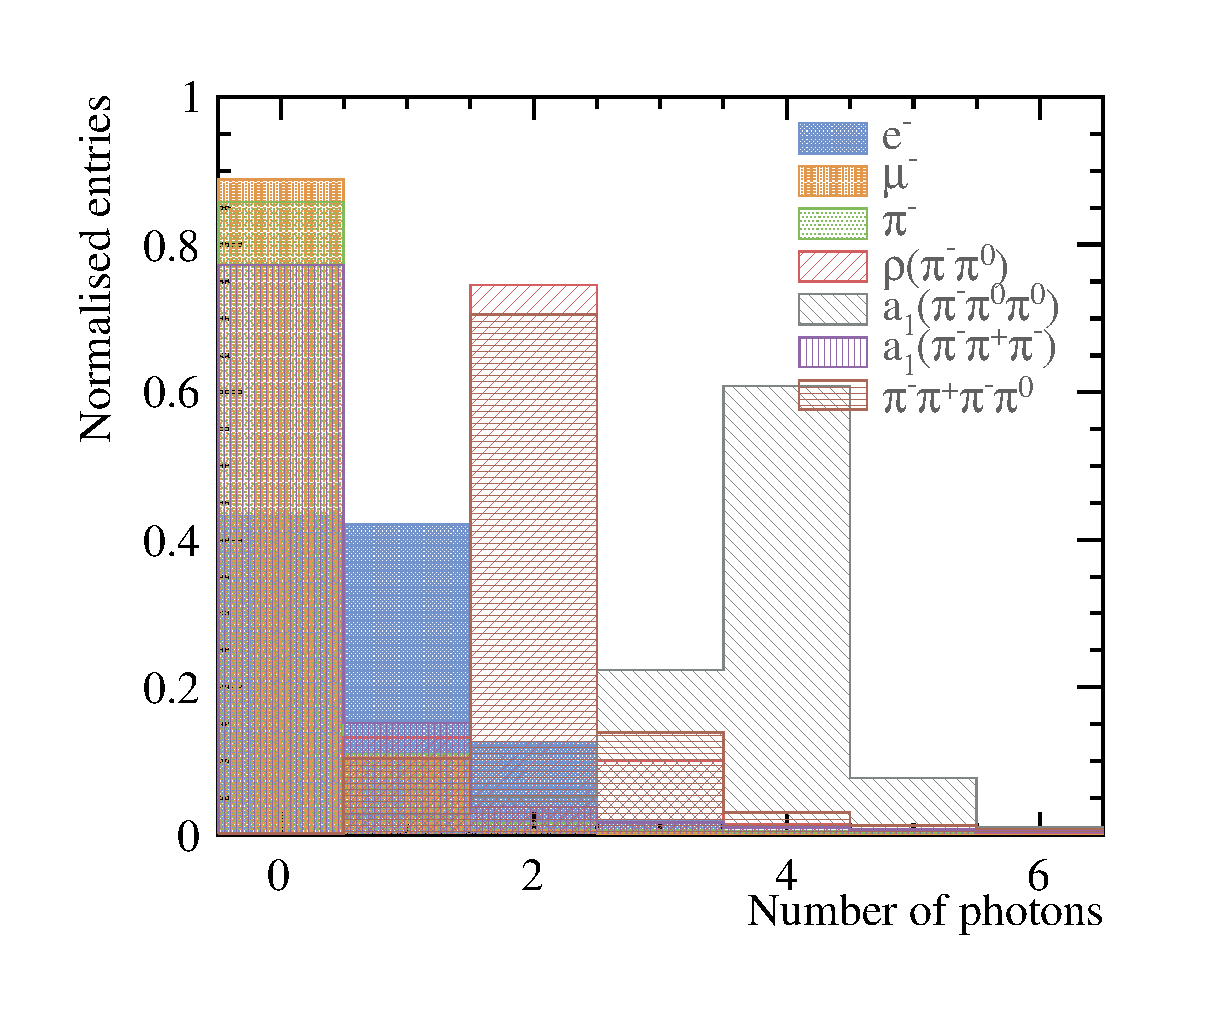
\includegraphics[width=.45\textwidth]{tau/var/nPhoton_100GeV_improved}
\qquad
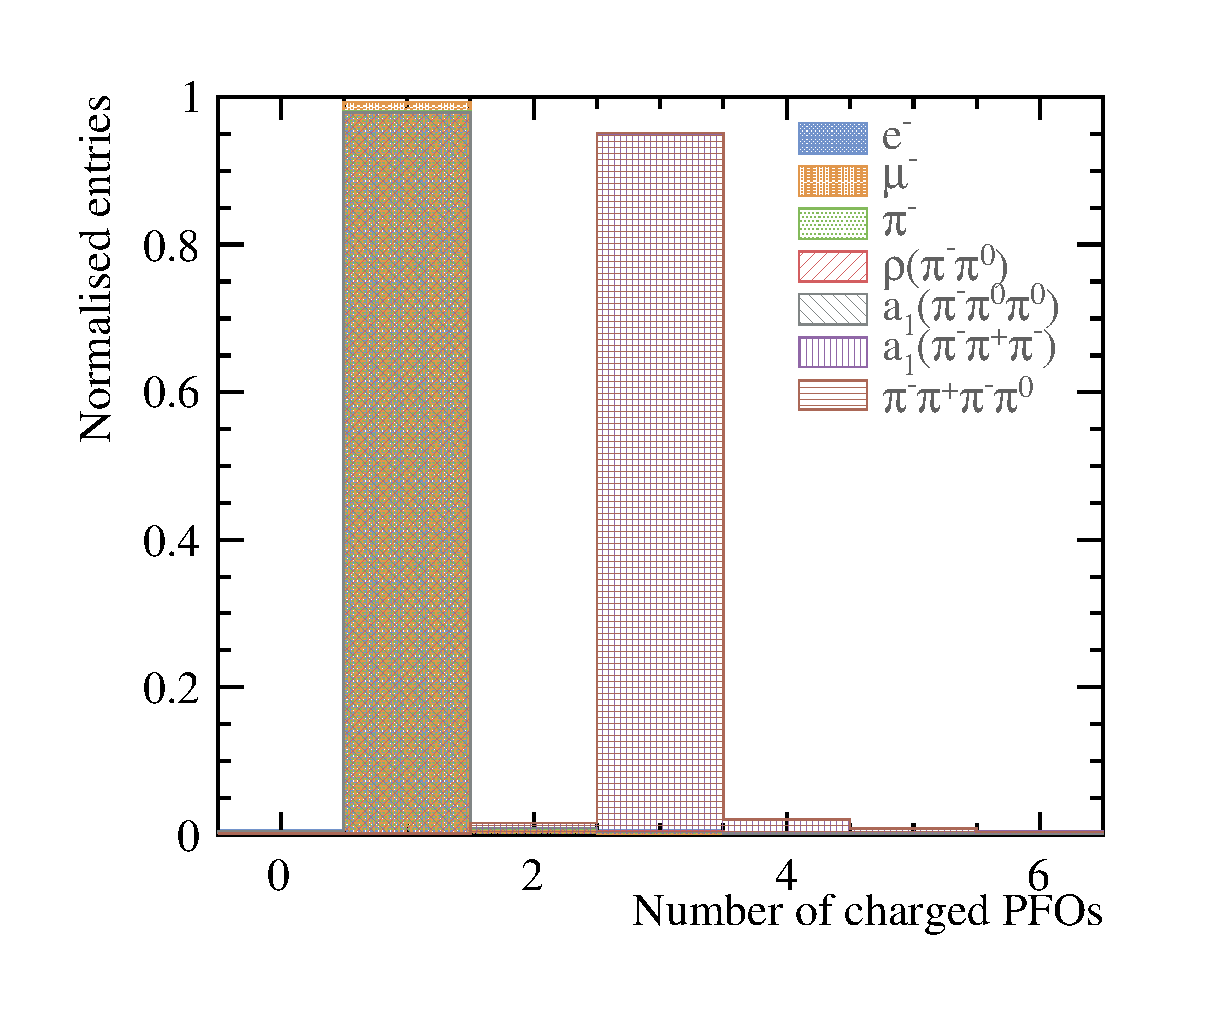
\includegraphics[width=.45\textwidth]{tau/var/nCharge_100GeV_improved}
\qquad
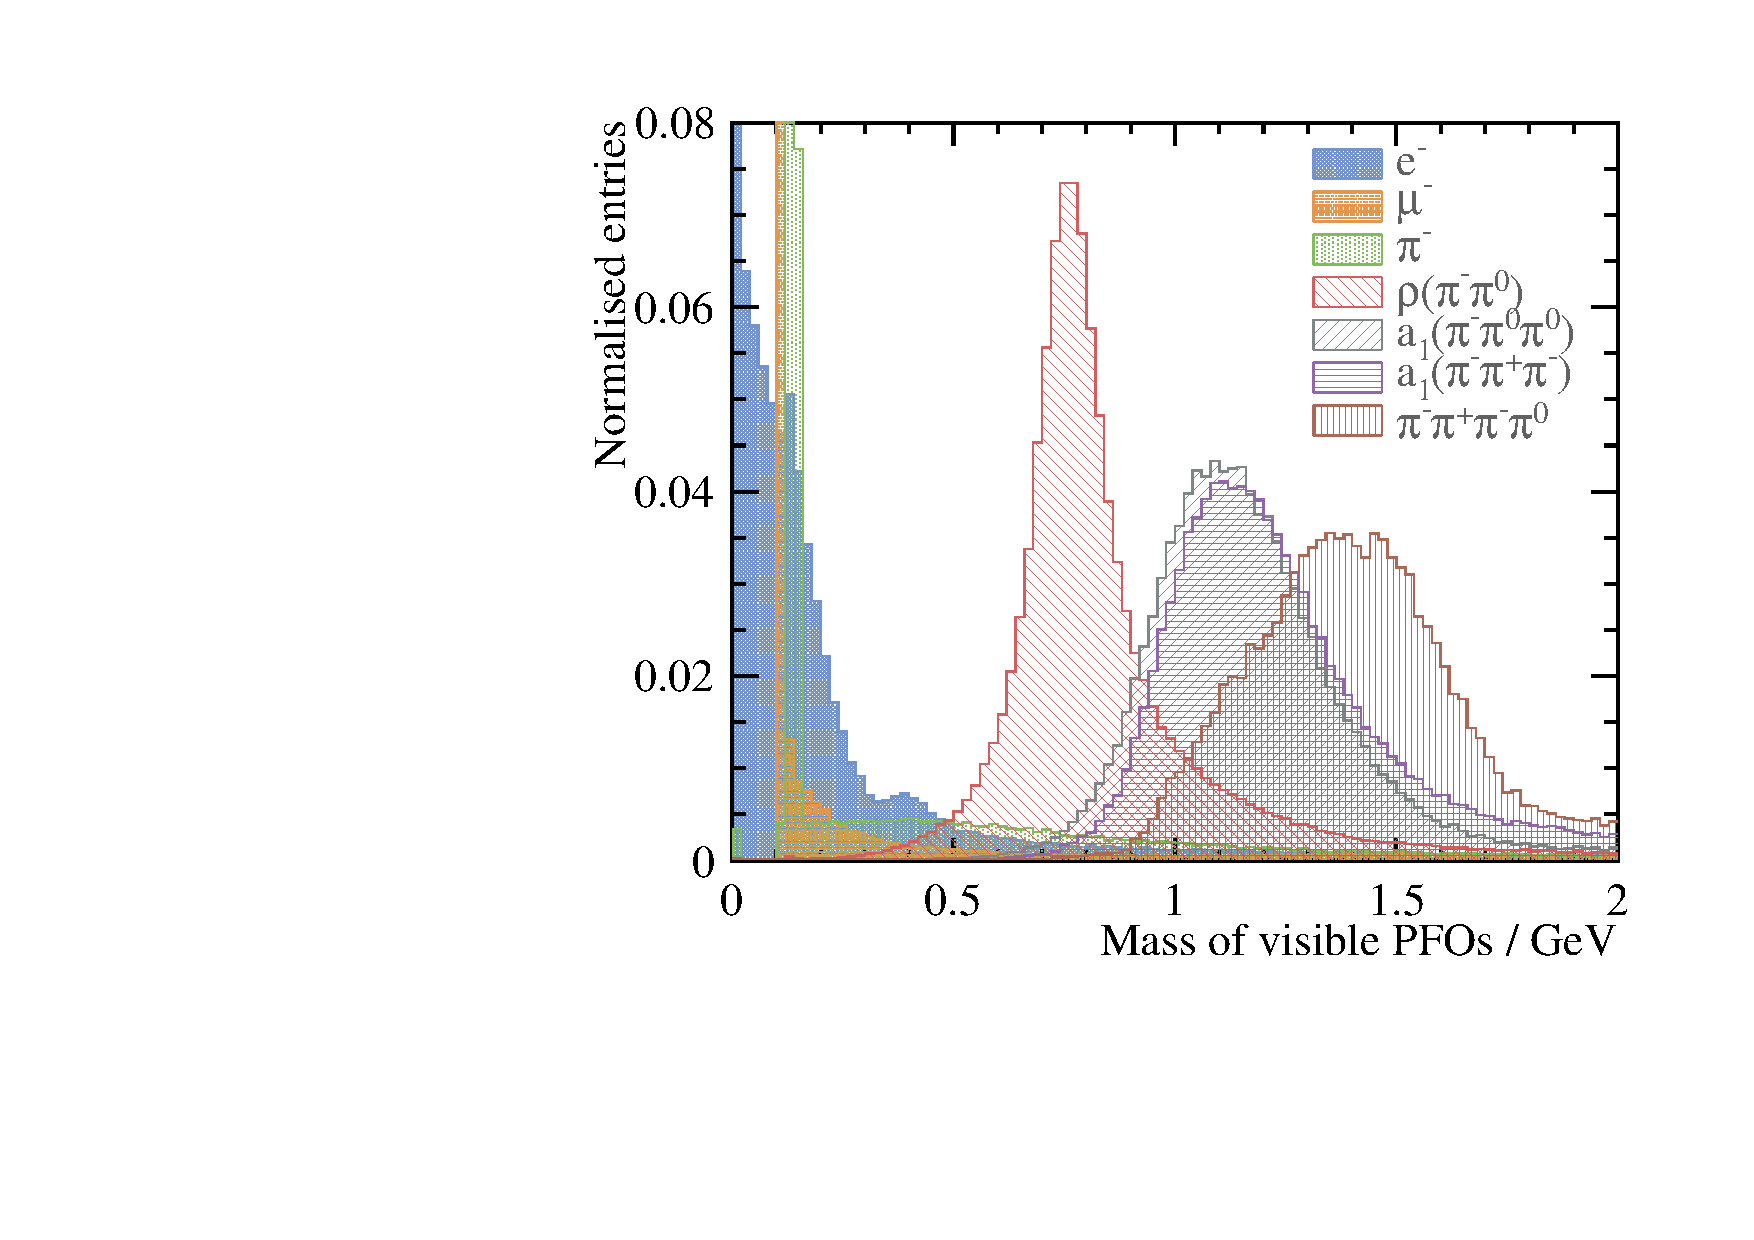
\includegraphics[width=.45\textwidth]{tau/var/mVis_100GeV_improved_zoom}
\qquad
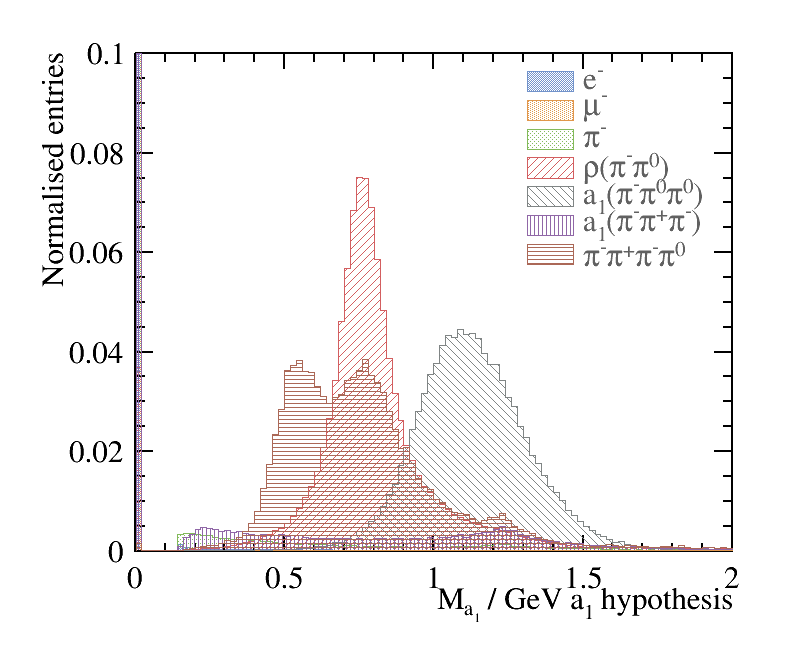
\includegraphics[width=.45\textwidth]{tau/var/mA1A1Fit_100GeV_improved_zoom}
\qquad

\caption[]{
Normalised distribution for selected discriminative variables for seven final states, \decayElectron, \decayMuon, \decayPion, \decayRho, \decayAiPhoton, \decayAiPion and \decayThreePionPhoton, separated using truth information,  for \rootSGeV{100} for nominal \CLICILD detector model. The top left, top right, bottom left and bottom right plots are the normalised entries against the number of photons, number of charged PFOs, invariant mass of visible PFOs, and the invariant mass of \decayAiPhotonShort for hypothesis test, respectively. There is a clear distinction between different final states in each plot.
}
\label{fig:tauVar}
\end{figure}

Some variables with most discriminative power are shown in figure~\ref{fig:nPfos}. In total 29 variables used in the multivariate analysis. The reason for the large number of variables is due to training seven decay modes at once, which will be discussed later.

Here is a full list of all variables used in the multivariate analysis. Energy of the \Pgt is assume to be the same as the energy of \Pepm colliding beam, which is half of the \rootS energy. Recoil momenta were calculated assuming the \Pem\Pep collision happened at the centre of mass energy. Both assumptions are largely valid when there is no ISR contribution.

\begin{itemize}
\item  $\frac{E_{ECal,HCal}}{E_{tot}}, charged$:  Sum of energy deposited in ECal and HCal, divided by the energy of charged particles
\item  $\frac{E_{ECal,HCal}}{E_{tot}}, all$:  	 Sum of energy deposited in ECal and HCal, divided by the energy of all particles
\item  $m_{vis}$:     	 Invariant mass of visible particles in GeV
\item  $\frac{E_{vis}}{E_{\Ptauon}}$:	 Sum of energy of all particles, divided by the energy of \Ptauon
\item  $\frac{E_{charged}}{E_{\Ptauon}}$:	 Sum of energy of charged particles, divided by the energy of \Ptauon
\item  $\frac{E_{\Pgmm}}{E_{\Ptauon}}$:	 Sum of energy of muons, divided by the energy of \Ptauon
\item  $\frac{E_{\Pem}}{E_{\Ptauon}}$:	 Sum of energy of electrons, divided by the energy of \Ptauon
\item  $\frac{E_{\Pgg}}{E_{\Ptauon}}$:	 Sum of energy of photons, divided by the energy of \Ptauon
\item  $\frac{E_{\Pgpm}}{E_{\Ptauon}}$:	 Sum of energy of charged pions, divided by the energy of \Ptauon
\item  $N_{charged}$:	 Number of charged particles
\item  $N_{\Pgmm}$:	 Number of muons
\item  $N_{\Pem}$:	 Number of electrons
\item  $N_{\Pgg}$:	 Number of photons
\item  $N_{\Pgpm}$:	 Number of charged pions
\item  $m_{\Pgg}$:     	 Invariant mass of photons in GeV
\item  $m_{charged}$:     	 Invariant mass of charged particles in GeV
\item  $m_{neutral}$:     	 Invariant mass of neutral particles in GeV
\item  $m_{\Pgpm}$:     	 Invariant mass of charged pions in GeV
\item  $m_{\Pgpz}, \decayRhoShort hypothesis$:     	 Fitted invariant mass of \Pgpz for \decayRhoShort hypothesis test
\item  $m_{\decayRhoShort}, \decayRhoShort hypothesis$:     	 Fitted invariant mass of \decayRhoShort for \decayRhoShort hypothesis test

\item  $m_{\Pgpz1}, \decayAiPhotonShort hypothesis$:     	 First fitted invariant mass of \Pgpz, for \decayAiPhotonShort hypothesis test, ordered by closeness to the true \Pgpz mass
\item  $m_{\Pgpz2}, \decayAiPhotonShort hypothesis$:     	 Second fitted invariant mass of \Pgpz, for \decayAiPhotonShort hypothesis test, ordered by closeness to the true \Pgpz mass
\item  $m_{\decayAiPhotonShort}, \decayAiPhotonShort hypothesis$:     	 Second fitted invariant mass of \decayAiPhotonShort, for \decayAiPhotonShort hypothesis test
\item  $\bar{E_{cell}}$:     	 Average energy deposited in a calorimeter cell in GeV
\item  $d_{trans,shower}$:    Transverse shower width for electromagnetic shower profile, averaged for all clusters in the ECal
\item  $l_{long,shower}$:    Longitudinal start layer for electromagnetic shower profile, averaged for all clusters in the ECal
\item  $\Delta{l_{long,shower}}$:    Longitudinal discrepancy for electromagnetic shower profile, averaged for all clusters in the ECal
\item  $\%MIP$:    Fraction of calorimeter hits registered as minimum ionised particles, averaged for all clusters in the ECal
\item  $\frac{E}{P}$:   Energy divided by momentum, averaged for all clusters in the ECal
\end{itemize}

Number of photons is an important variable for separating decay modes. This information is only available due to the excellent photon reconstruction. Shown in \Figure{fig:nPfos}, the majority of \decayMuon, \decayPion and \decayAiPion final states have zero photon reconstructed. The \decayElectron final state event have one photon reconstructed instead of zero, due to the FSR effect. \decayRho and \decayThreePionPhoton have nearly 80\% events with two reconstructed photons, whilst \decayAiPion have over 60\% events with four reconstructed photons. The loss is efficiency is due to the increasing difficulty to separate nearby photons.

The number of charged PFOs can clearly separate the leptonic and 1-prong final states, from the 3-prong final states, shown in \Figure{fig:nPfos}. The efficiency of leptonic final states are over 98\%.

The invariant mass of the visible PFOs shows clear differences between different final states. \decayRho, \decayAiPhoton and \decayAiPion distribution show clear resonance at \Prho and \Pai. \decayElectron, \decayMuon and \decayPion distribution show much smaller invariant mass and \decayThreePionPhoton shows a large invariant mass than \Pai. The \decayElectron final state has a long tail of invariant mass due to the extra photons from the FSR.

$\frac{E_{ECal,HCal}}{E_{tot}}, charged$ and $\frac{E_{ECal,HCal}}{E_{tot}}, all$ are both very effective at picking out leptonic decay modes.

For final states containing \Prho and \Pai resonance, it is useful to use minimisation test for right pairing of the resonance. We will use \decayAiPhotonShort as an example. \decayRhoShort is very similar.

The minimisation of \decayAiPhotonShort hypothesis states

\begin{equation}
\label{eq:a1}
\chi_{\Pai}^{2} = {\left(\frac{m_{\Pai,fit} -  m_{\Pai}}{\sigma_{\Pai}}\right)}^{2} + {\left(\frac{{m_{\Pgpz,fit}} -  m_{\Pgpz}}{\sigma_{\Pgpz}}\right)}^{2} + {\left(\frac{{m_{\Pgpz^*,fit}} -  m_{\Pgpz}}{\sigma_{\Pgpz}}\right)}^{2}  \,,
\end{equation}

where $m_{\Pgpz,fit}$ and $m_{\Pgpz^*,fit}$  are the invariant masses of all possible two photons combinations, $\sigma_{\Pai}$ and $\sigma_{\Pgpz}$ are the half width of the invariant mass distribution of reconstructed \Pai and \Pgpz using the truth information, and $m_{\Pai}$ and $m_{\Pgp}$ are the masses of \Pai and \Pgpz, taken from \cite{Agashe:2014kda}. If there are only two or three photons, the $\chi_{\Pai}^{2}$ expression will be reduced and not including $m_{\Pgpz^*,fit}$ term, assuming two photons are merged in the reconstruction. If there are fewer than two photons, the $\chi_{\Pai}^{2}$ expression would only contain $m_{\Pai,fit}$ term.

For the \decayRho final state, a similar $\chi_{\Pgri}^{2}$ test for \Pgri hypothesis is used to extract $m_{\Pgri,fit}$ and $m_{\Pgpz,fit}$ variables. $\chi_{\Pgri}^{2}$ is similar to $\chi_{\Pai}^{2}$ with \Pgri replacing \Pai and only one $m_{\Pgpz,fit}$ term.


\Figure{fig:nPfos} shows the $m_{\Pai,fit}$ where \decayRho, \decayAiPhoton  and \decayThreePionPhoton final states contribute to the \Pai resonance, although only \decayAiPhoton final has a real \Pai resonance. This is due to the structure of the  $\chi_{\Pai}^{2}$ minimisation function allowing final states with more than two photons and one \Pgppm to contribute.

Last six variables in the list help to differentiate an electron final state to that of a charged pion. A charged pion that starts showering early in the calorimeter could have a similar topology to an electromagnetic shower. Nevertheless, a good separation between the two can be achieved with the help of these variables.

\section{Multivariate Analysis}

For the multivariate analysis, the multiclass class of the TMVA package \cite{Therhaag:2009dp} was used to perform a multiclass classification, which trains the seven final states simultaneously. The multiclass class is an extension of the standard two-class signal-background classifier.

There are two ways for the training. "One v.s. one" is each class is trained against each other class. And the overall likelihood is normalised. The second way to train is called "one v.s. all", which is when each class is trained against all other classes.

Using a three-class example, A, B and C, "one v.s. one" scheme trains A against B, B against C, and C against A. Then the likelihood is normalised. "One v.s. all" would train A against B plus C, B against A plus C, and C against A plus B.

TMVA multiclass implementation uses "one v.s. all" scheme. For each final state, the multiclass classifier will train the final state as the signal against all other final states as the background. This process is repeated for each final state. The classifier output for a single event is a normalised response for each final state, where the sum is one. The response of each final state of a event can be treated as the likelihood. The event is classified into a particular final state if the final state has the highest classifier output response. The advantage of using the multiclass is that the correlation between different final states are accounted for and the classifier output are correctly adjusted for multiple final states, hence one event can only be classified into one final state. The issue with the multiclass is that discriminative variables for each final state need enter the training stage, resulting in a large number of variables.

Half of the randomly selected samples were used in the training process and the other half were used for testing.

The TMVA multiclass classifier used is boosted decision tree with gradient boosting (BDTG), as it was found to give for the best performance. The MVA classifier is trained and optimised to give the best overall separation across all final states. MVA will be discuss further in \Section{}

\section{Result}


\begin{table}[htbp]
\centering

\smallskip
\small
\begin{tabular}{| l | r | r | r | r | r | r | r |}
\hline
  Reco $\downarrow$ True $\to$  & \decayElectronShort & \decayMuonShort &\decayPionShort & \decayRhoShortest &\decayAiPhotonShortest &\decayAiPionShortest &\decayThreePionPhotonShort \\
\hline

\decayElectronShort  &\textbf{99.8}&-&0.9&1.1&0.8&-&-\\
\decayMuonShort   &-&\textbf{99.5}&0.5&-&-&-&-\\
\decayPionShort  &-&0.3&\textbf{93.2}&0.9&-&0.4&-\\
\decayRhoShortest&-&-&4.1&\textbf{93.0}&10.5&0.6&2.8\\
\decayAiPhotonShortest&-&-&-&4.3&\textbf{88.2}&-&1.0\\
\decayAiPionShortest&-&-&1.0&0.3&-&\textbf{96.6}&6.9\\
\decayThreePionPhotonShort&-&-&-&0.4&0.4&2.4&\textbf{89.3}\\

\hline
\end{tabular}

\caption[]%
{The percentage of reconstructed decay modes corresponds to underlying true decay modes, with \rootSGeV{100} for nominal \CLICILD detector model. Bold numbers show the correctly reconstructed percentages. Numbers less than 0.25\% are not shown. Statistical uncertainties are less than 0.25\%. Final states include \Pgngt, which is not shown.}
\label{tab:TauSelExample}
\end{table} 


The reconstruction efficiencies for the seven final state of the tau decaying with c.o.m. energy of 100 \,GeV for the nominal CLIC\_ILD detector are shown in \Table{tab:TauSelExample}. The perfect reconstruction would result in only terms in the diagonal.

The unprecedented high classification rate has been achieved. The improvement of photon reconstruction described in \Section{} improved the ability to separate 1-prong final state. Most notably,  \Figure{} shows number of photons have a high correct reconstruction efficiency.

For leptonic decay, the selection efficiency is above 99.5\% as the tracking system have much better resolution than the calorimeter.

The \decayMuonShort final state has very clear topology, as muon deposits energy in the muon chamber. Therefore, there is little confusion with other final states.

\decayElectronShort final state is well separated, due to the specialised variables aimed to differentiate early hadronic shower to electromagnetic shower. However, there is still about 1\% confusion in one prong final state.

For one prong final states, \decayPionShort, \decayRhoShortest, and \decayAiPhotonShortest, the confusion is mainly due to the imperfect separation of nearby photons, originated form \Ppizero. 


Similarly the confusion between 3-prong final state, \decayAiPionShortest, and \decayThreePionPhotonShort is caused by the inability to resolve photon pairs.

\section{Electromagnetic calorimeter  optimisaiton}

As discussed above, the tau decay mode separation is an benchmark test of detector performance. The ability to resolve photon pairs is crucial to separate different 1-prong states, and different 3-prong state. One of the main feature of calorimeter design affecting the photon resolution is the size of electromagnetic calorimeter (ECal) cell for the high granular calorimeter. The finer ECal cell size is, the better resolution of reconstructing individual photons.


The classification is being tested with the impact of different \sqrtS and different ECal square cell sizes. Around two million events were simulated at each \sqrtS = 100, 200, 500 and 1000\,GeV, with each different ECal square cell sizes of 3, 5, 7, 10, 15 and 20\,mm. Events were simulated and reconstructed in the same way as described above, with same selection applied. MVA classifier was trained individually for each \sqrtS and each ECal square cell size, with same set of discriminative variables.

\begin{figure}[htbp]
\centering % \begin{center}/\end{center} takes some additional vertical space
%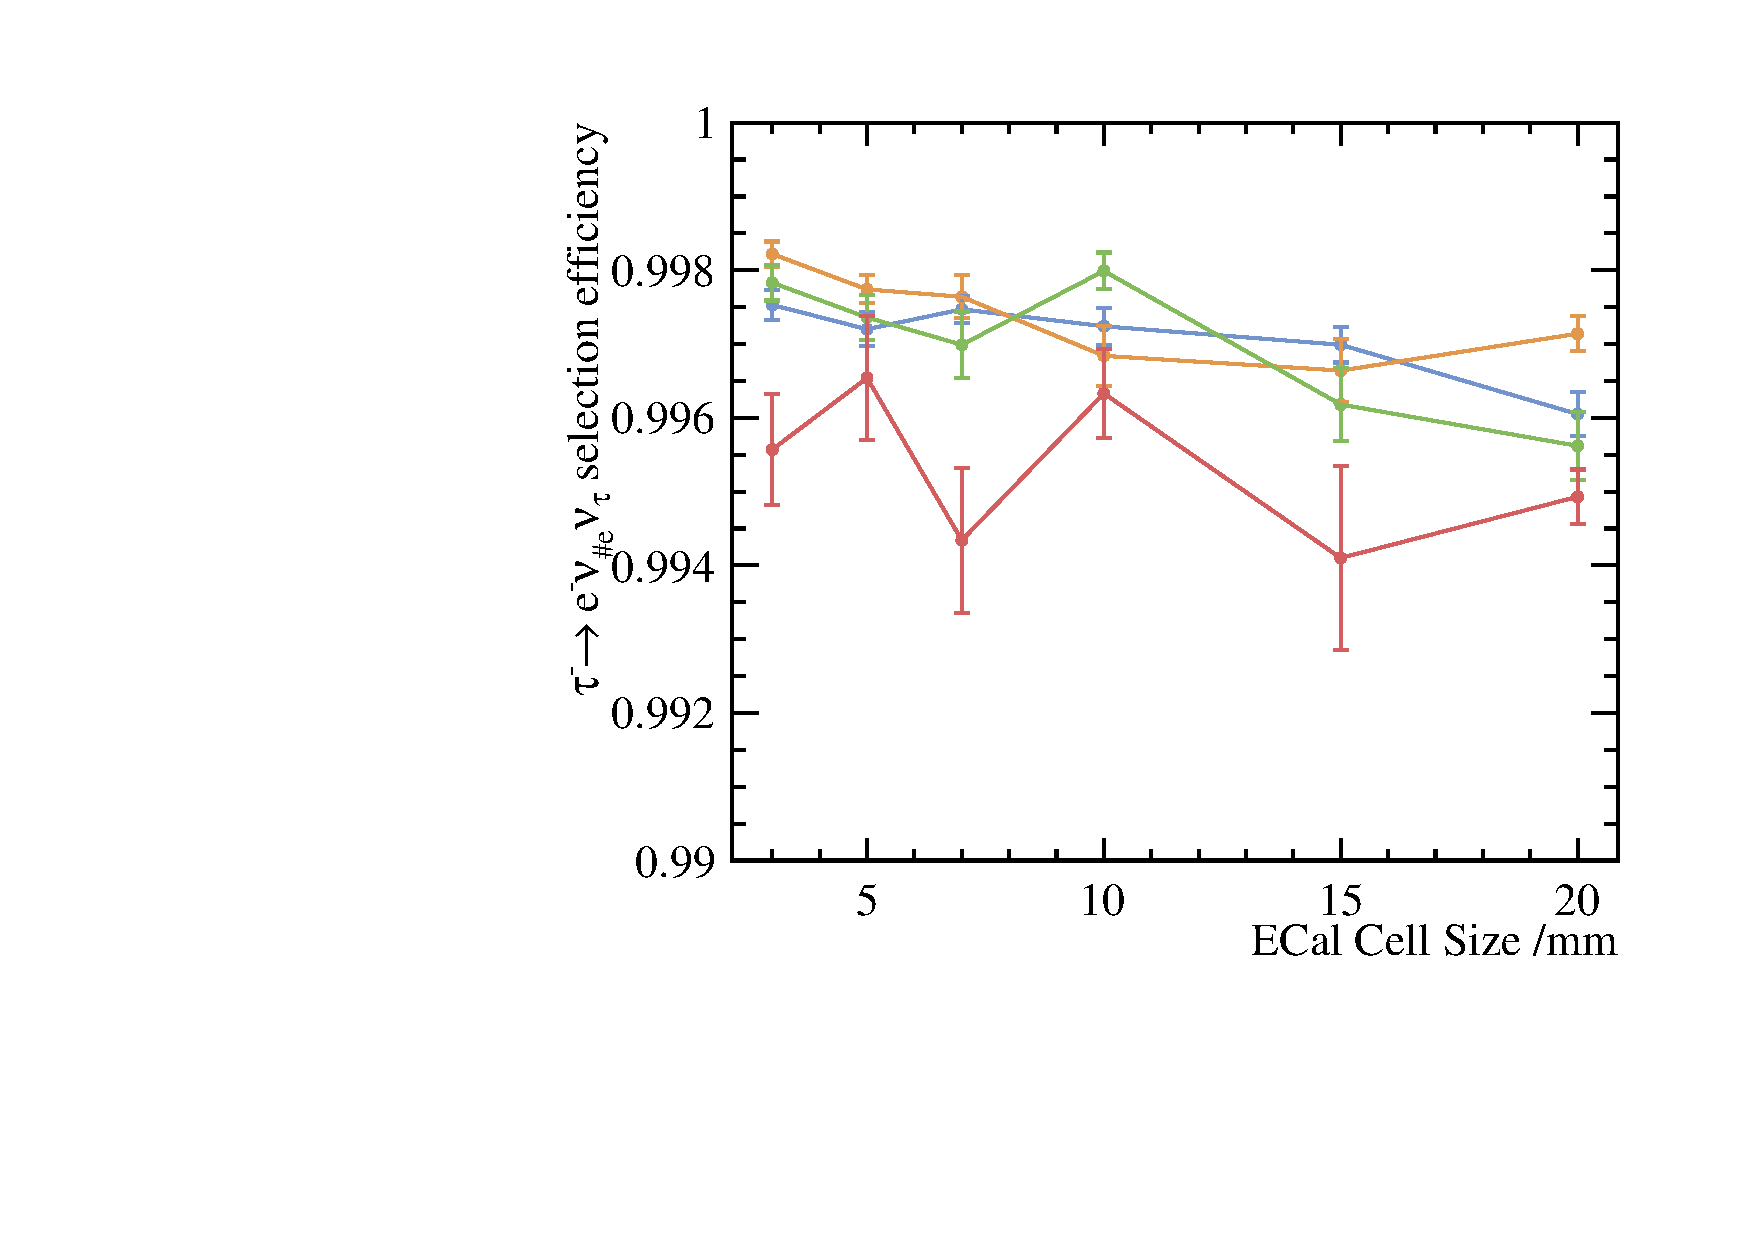
\includegraphics[width=.45\textwidth]{plots/decayMode0}
%\qquad
%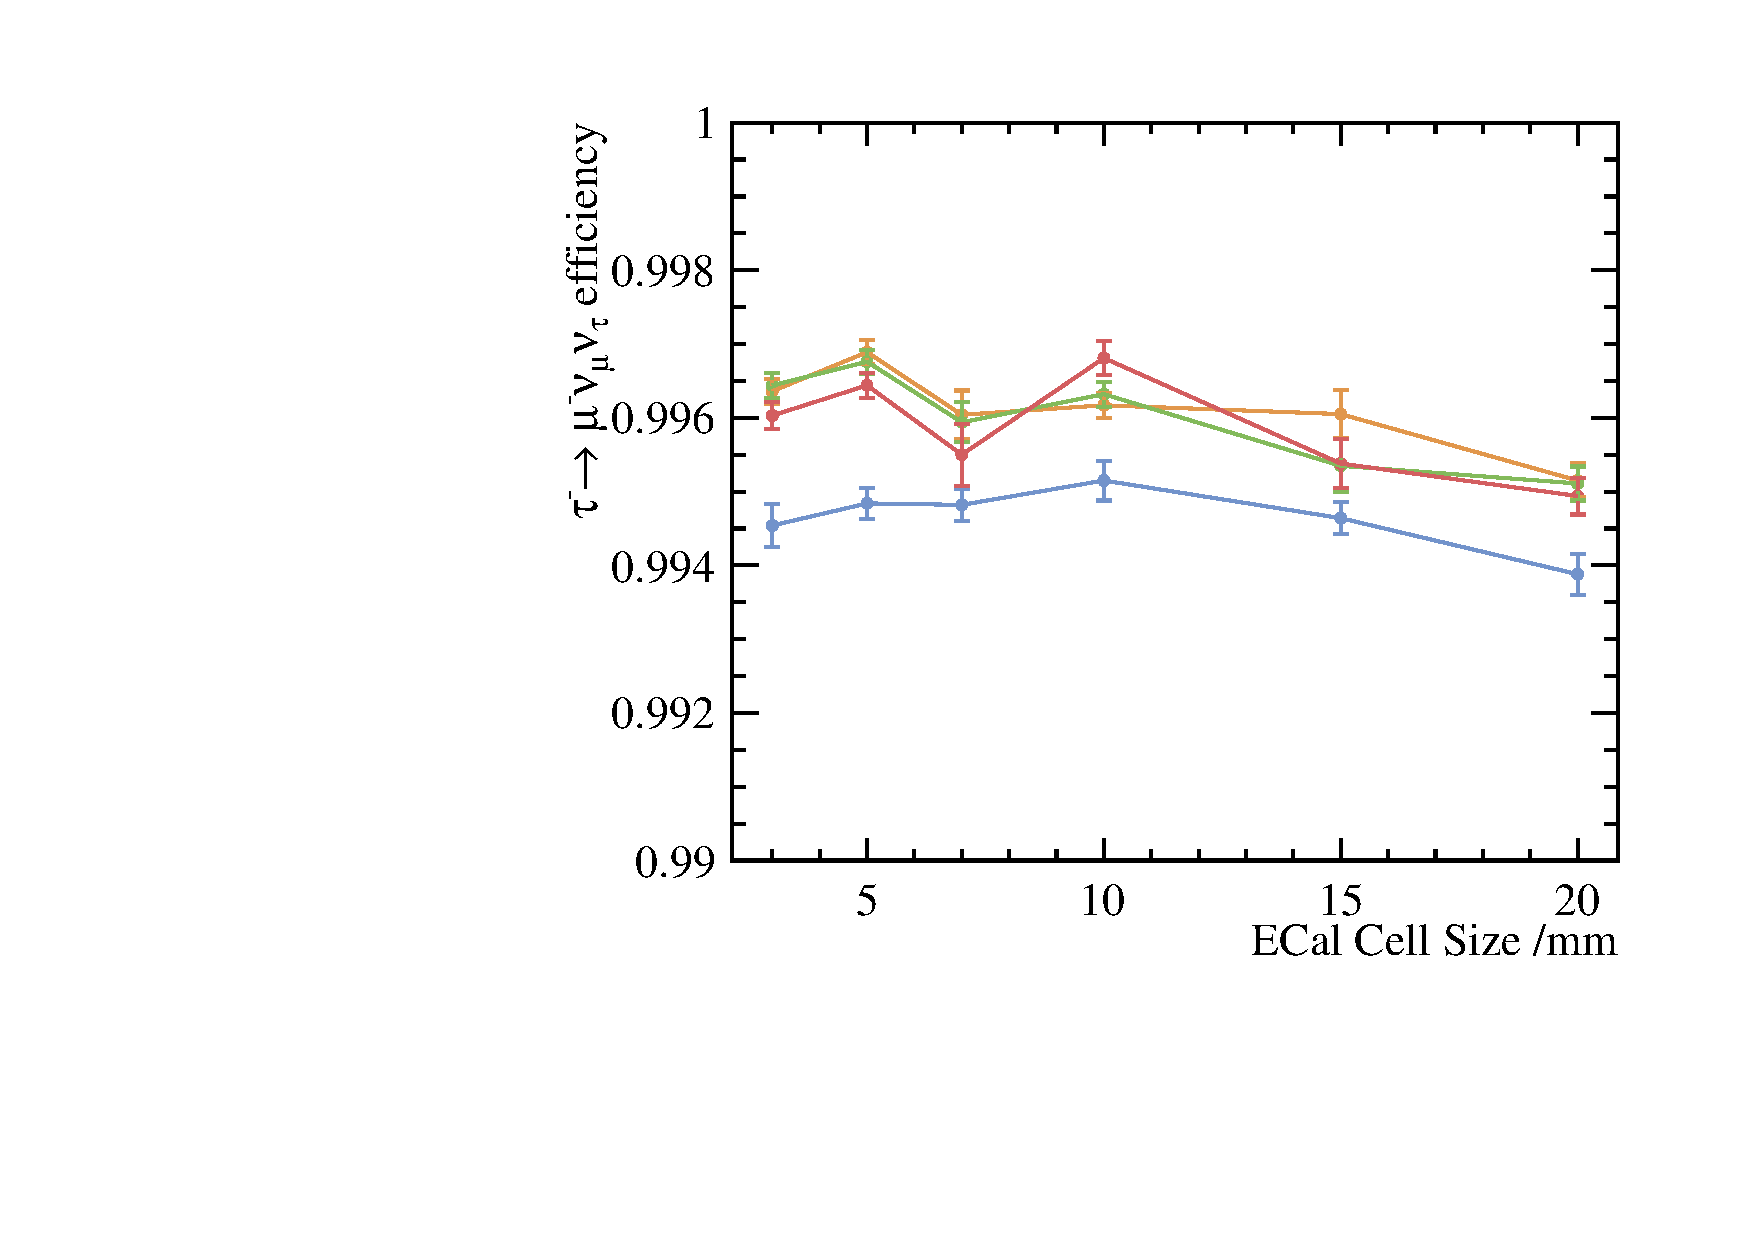
\includegraphics[width=.45\textwidth]{plots/decayMode1}
%\qquad
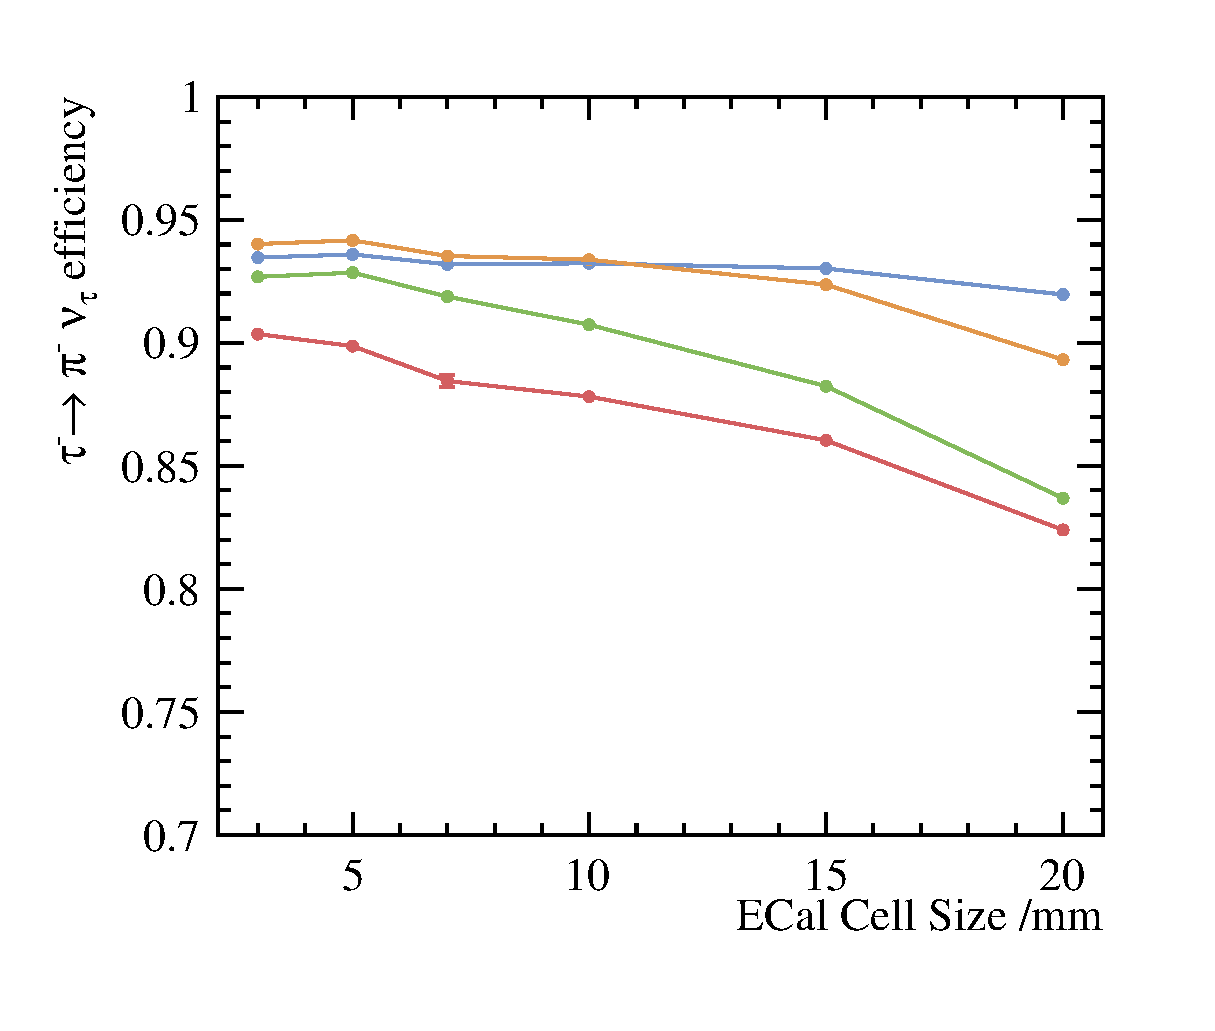
\includegraphics[width=.45\textwidth]{tau/decayMode2}
\qquad
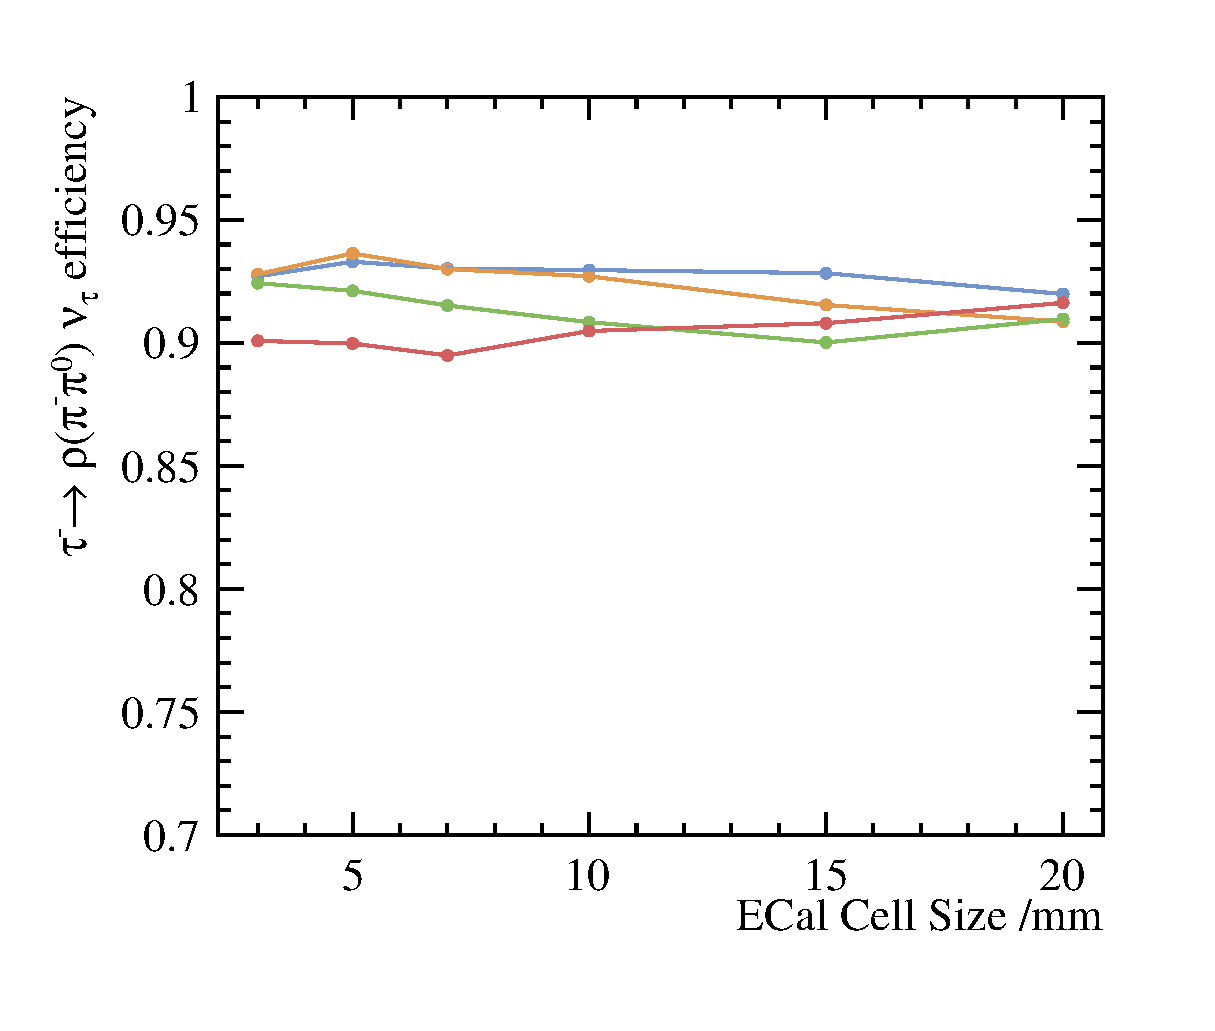
\includegraphics[width=.45\textwidth]{tau/decayMode3}
\qquad
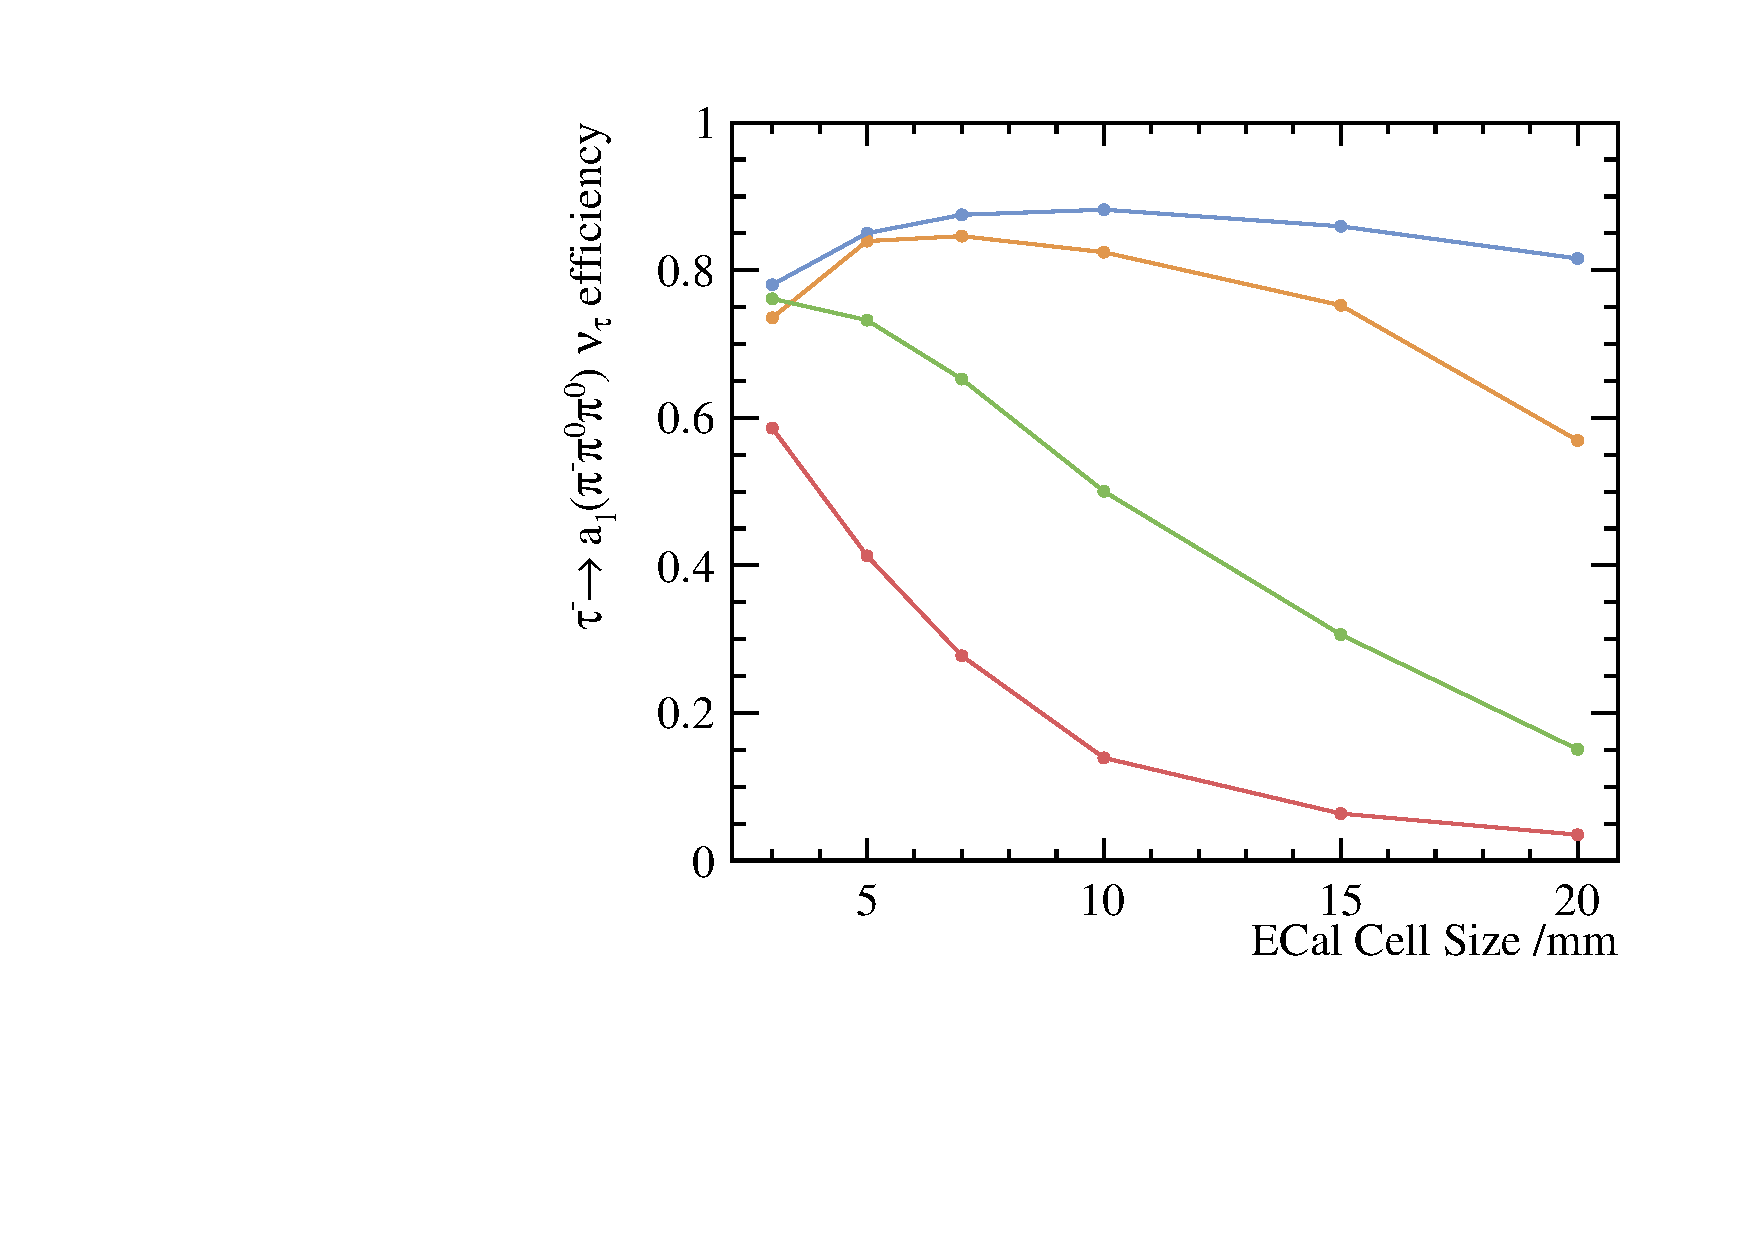
\includegraphics[width=.45\textwidth]{tau/decayMode4}
\qquad
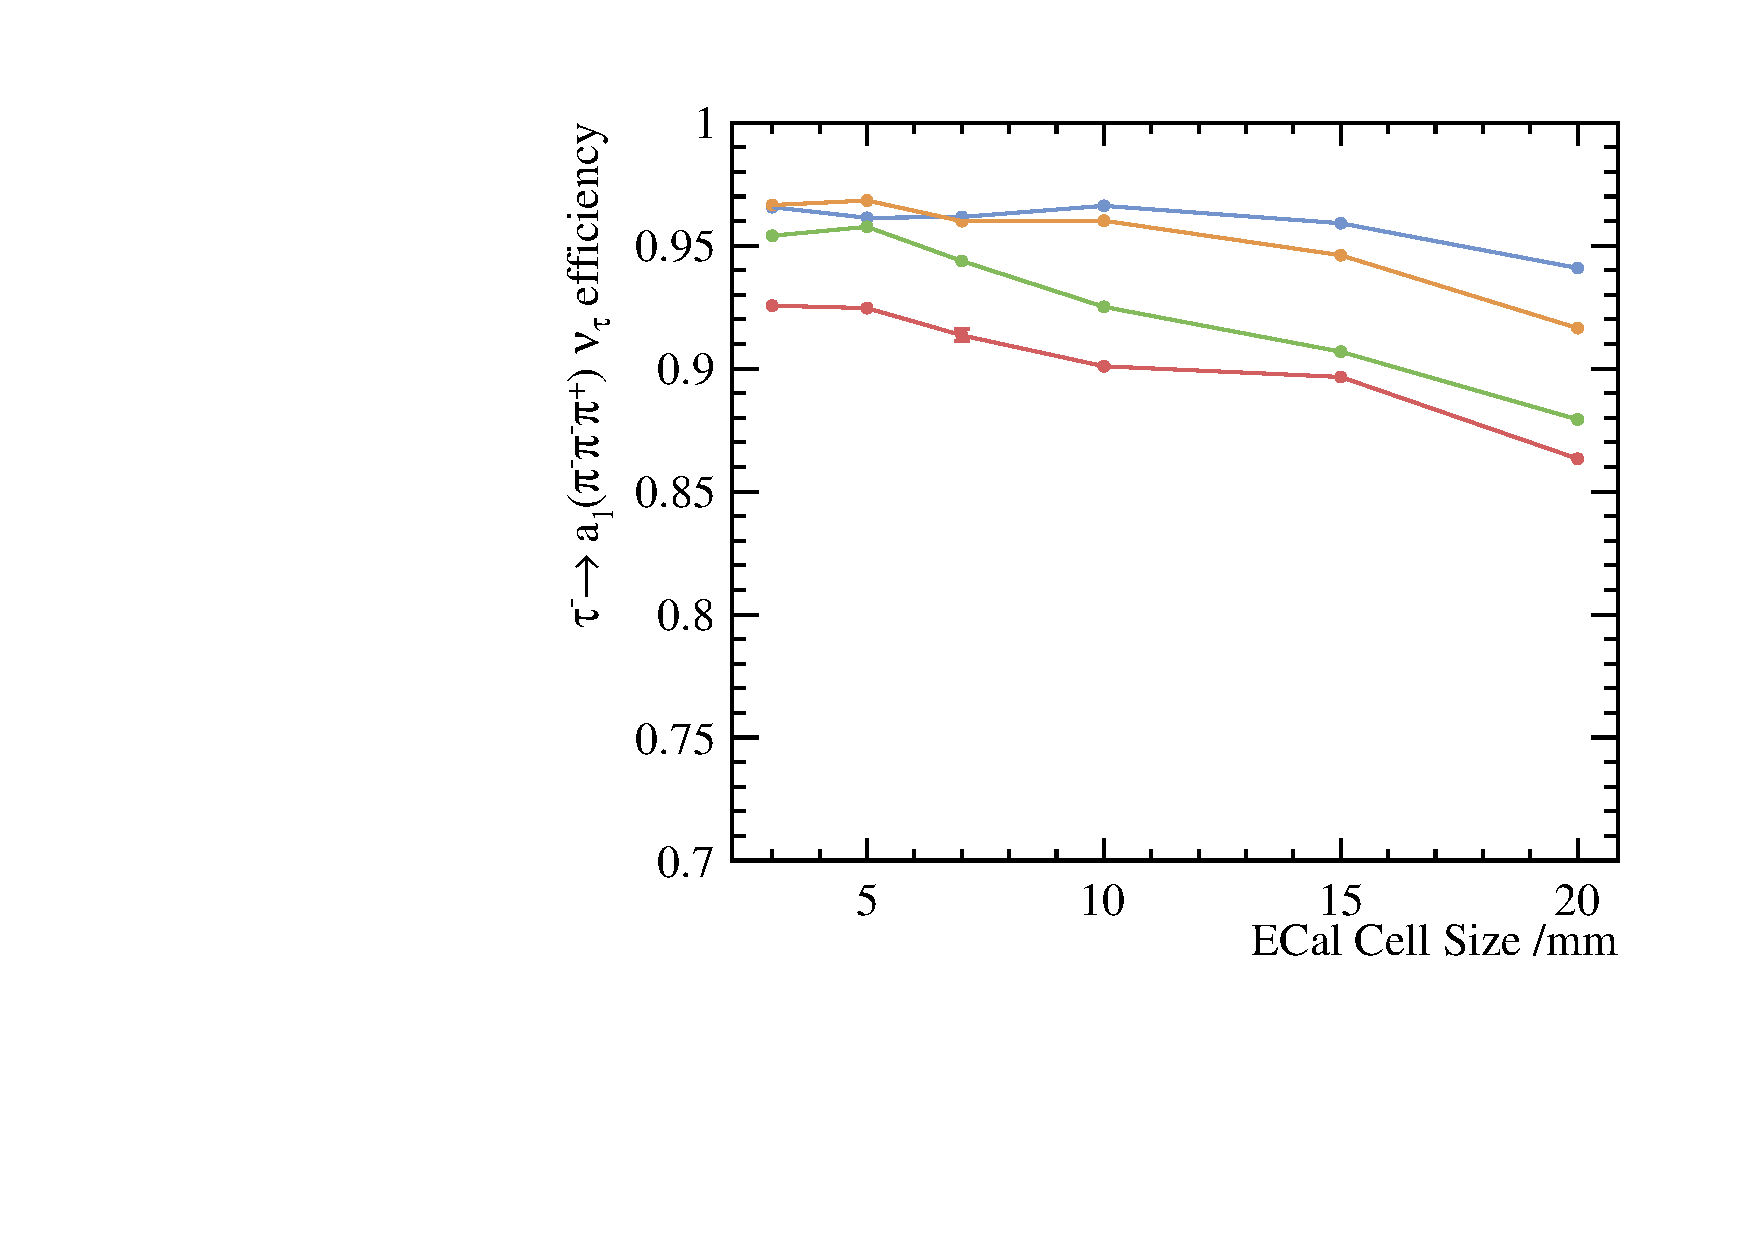
\includegraphics[width=.45\textwidth]{tau/decayMode5}
\qquad
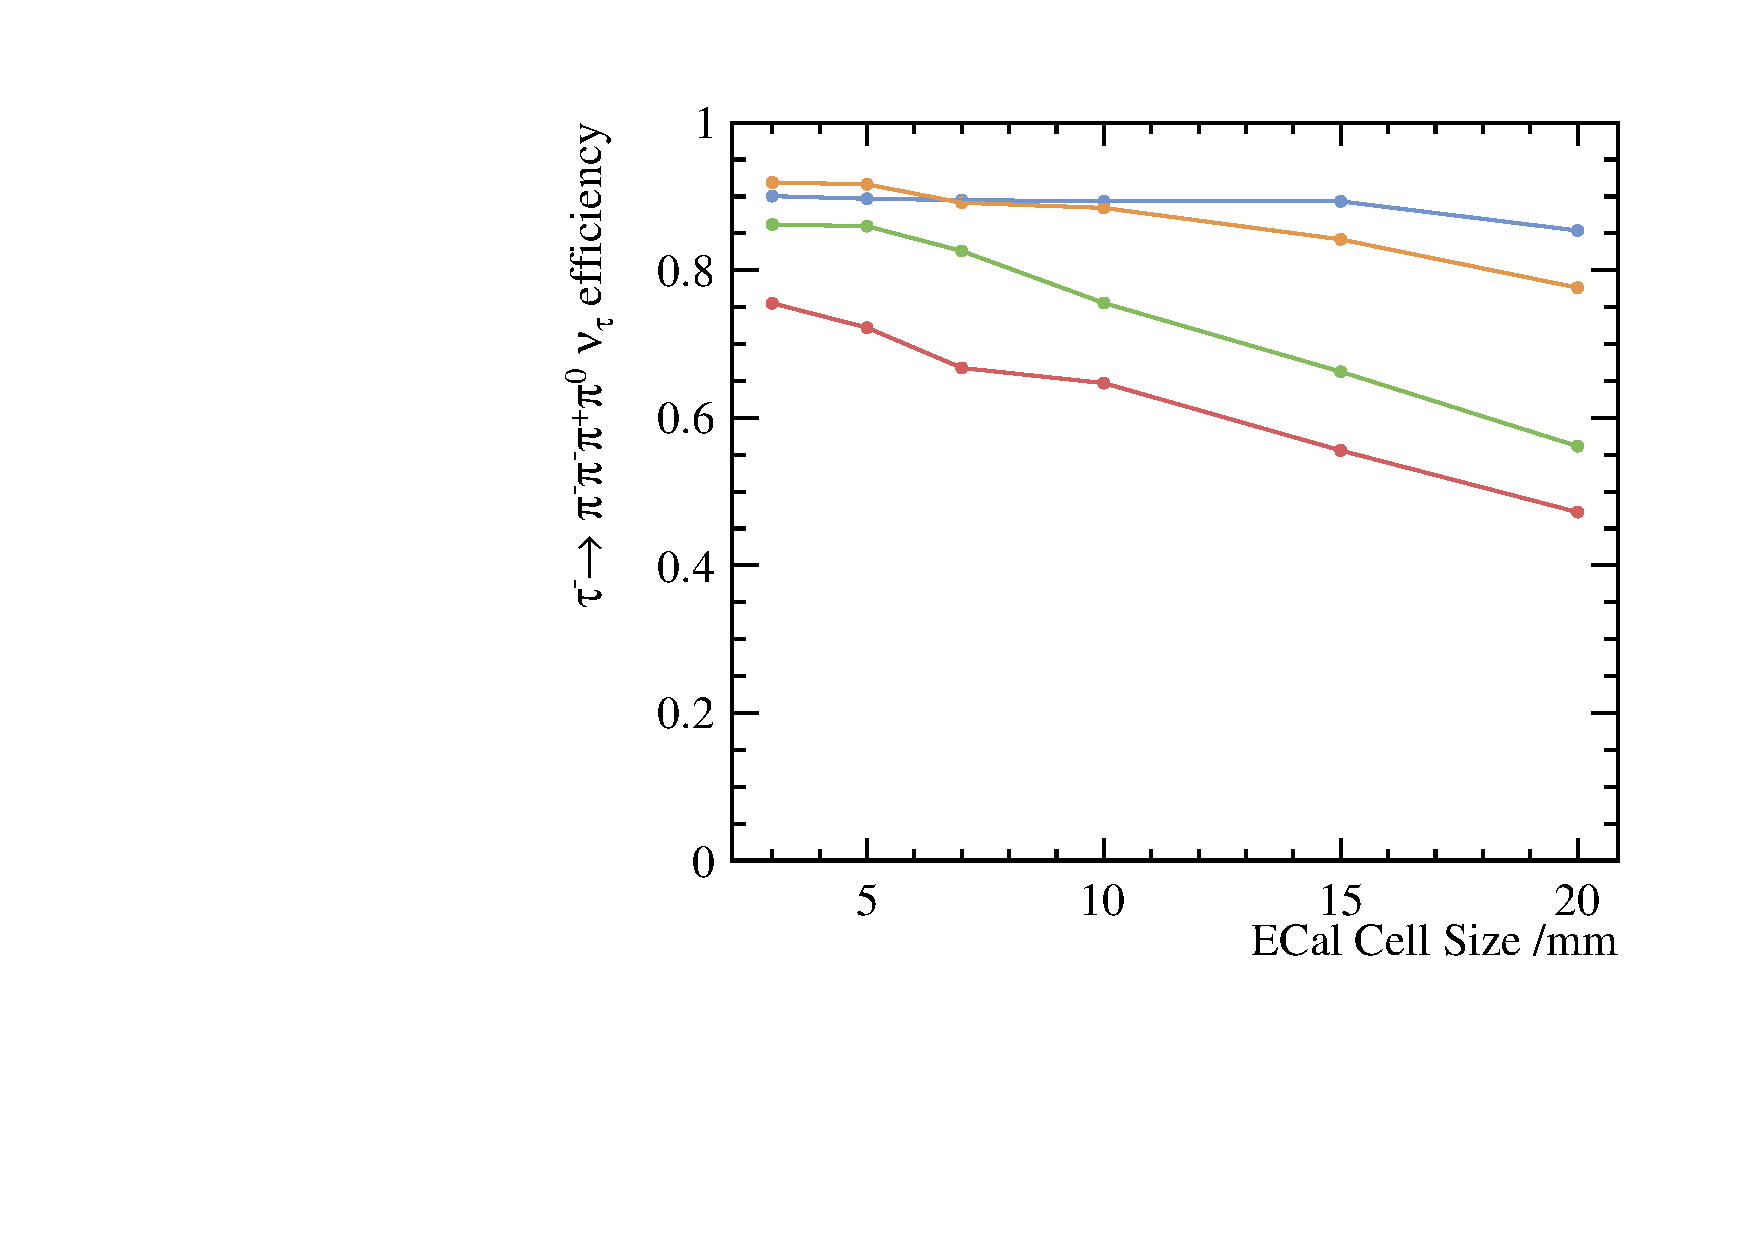
\includegraphics[width=.45\textwidth]{tau/decayMode6}
\qquad
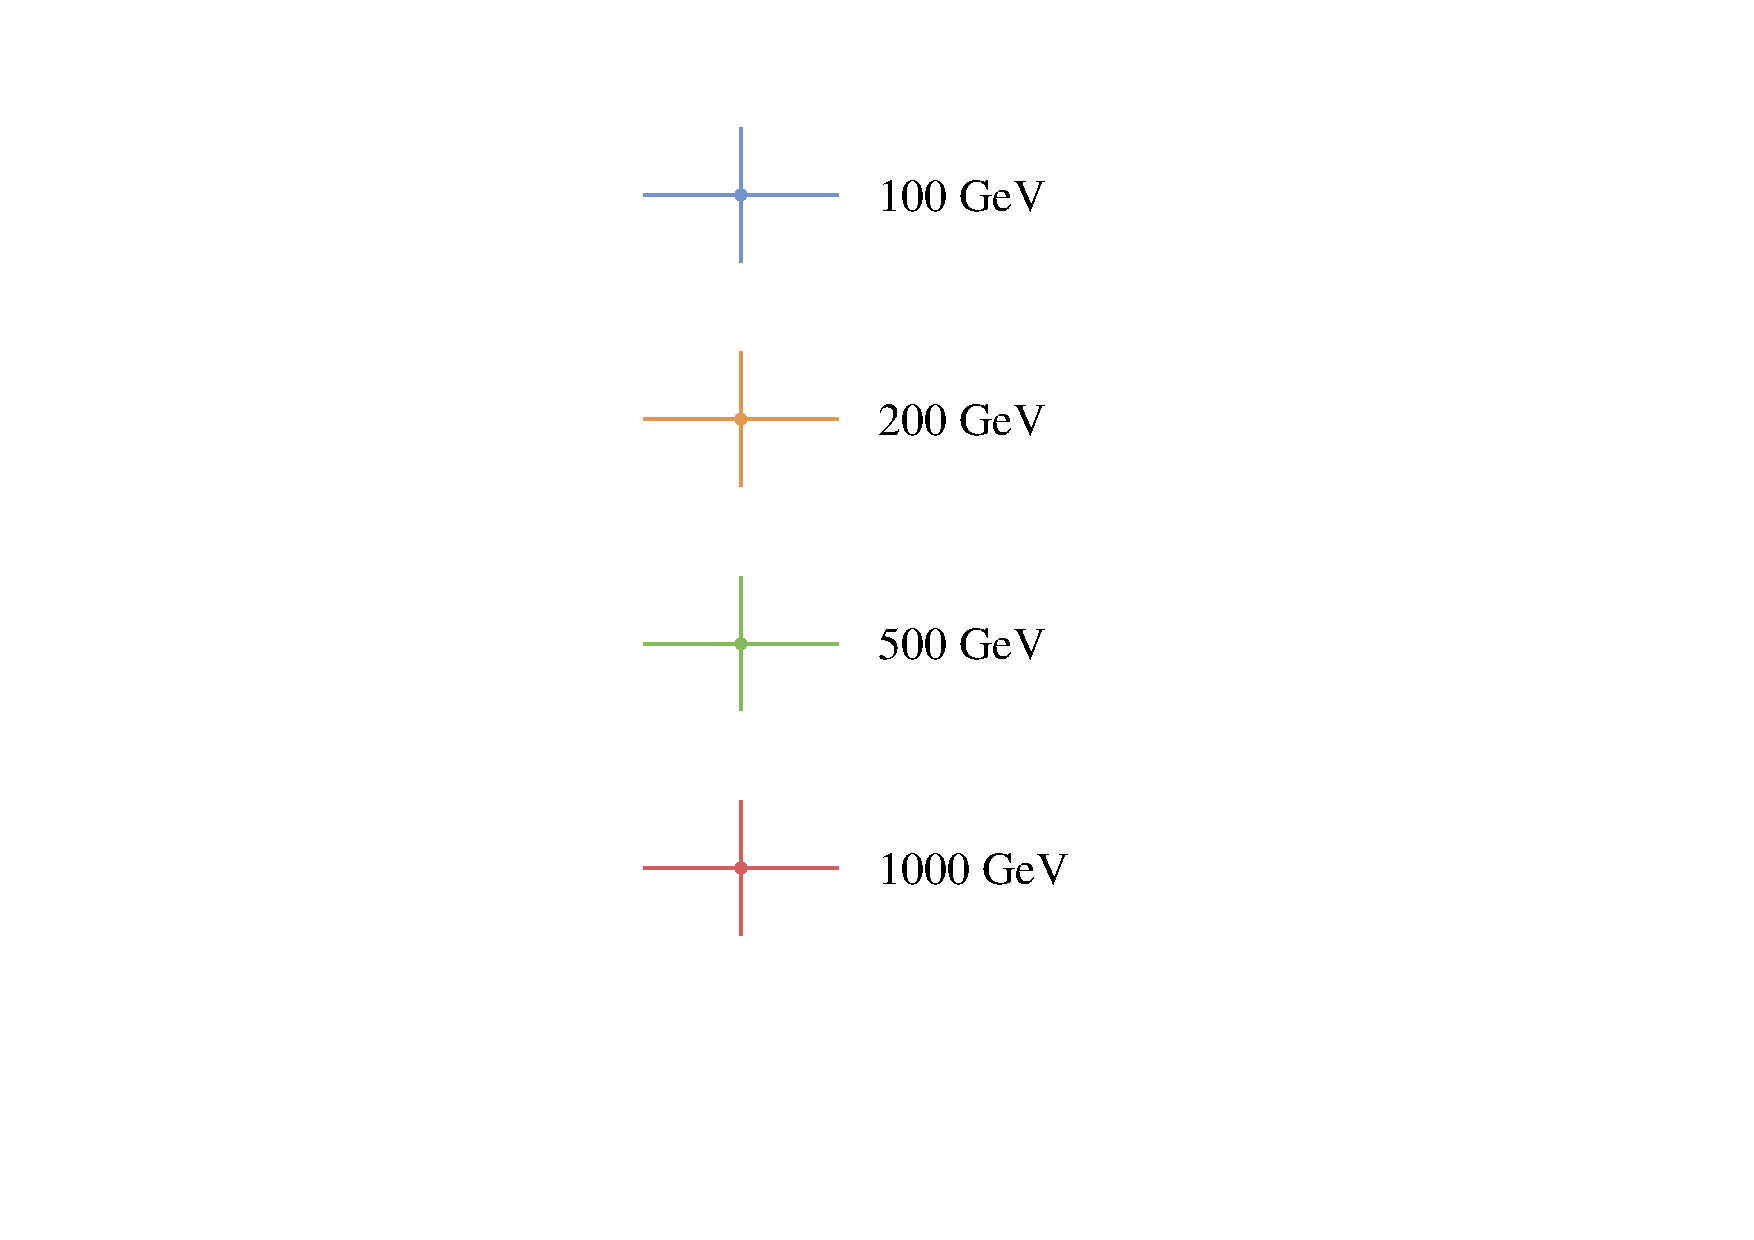
\includegraphics[width=.45\textwidth]{tau/legend}
%\qquad
%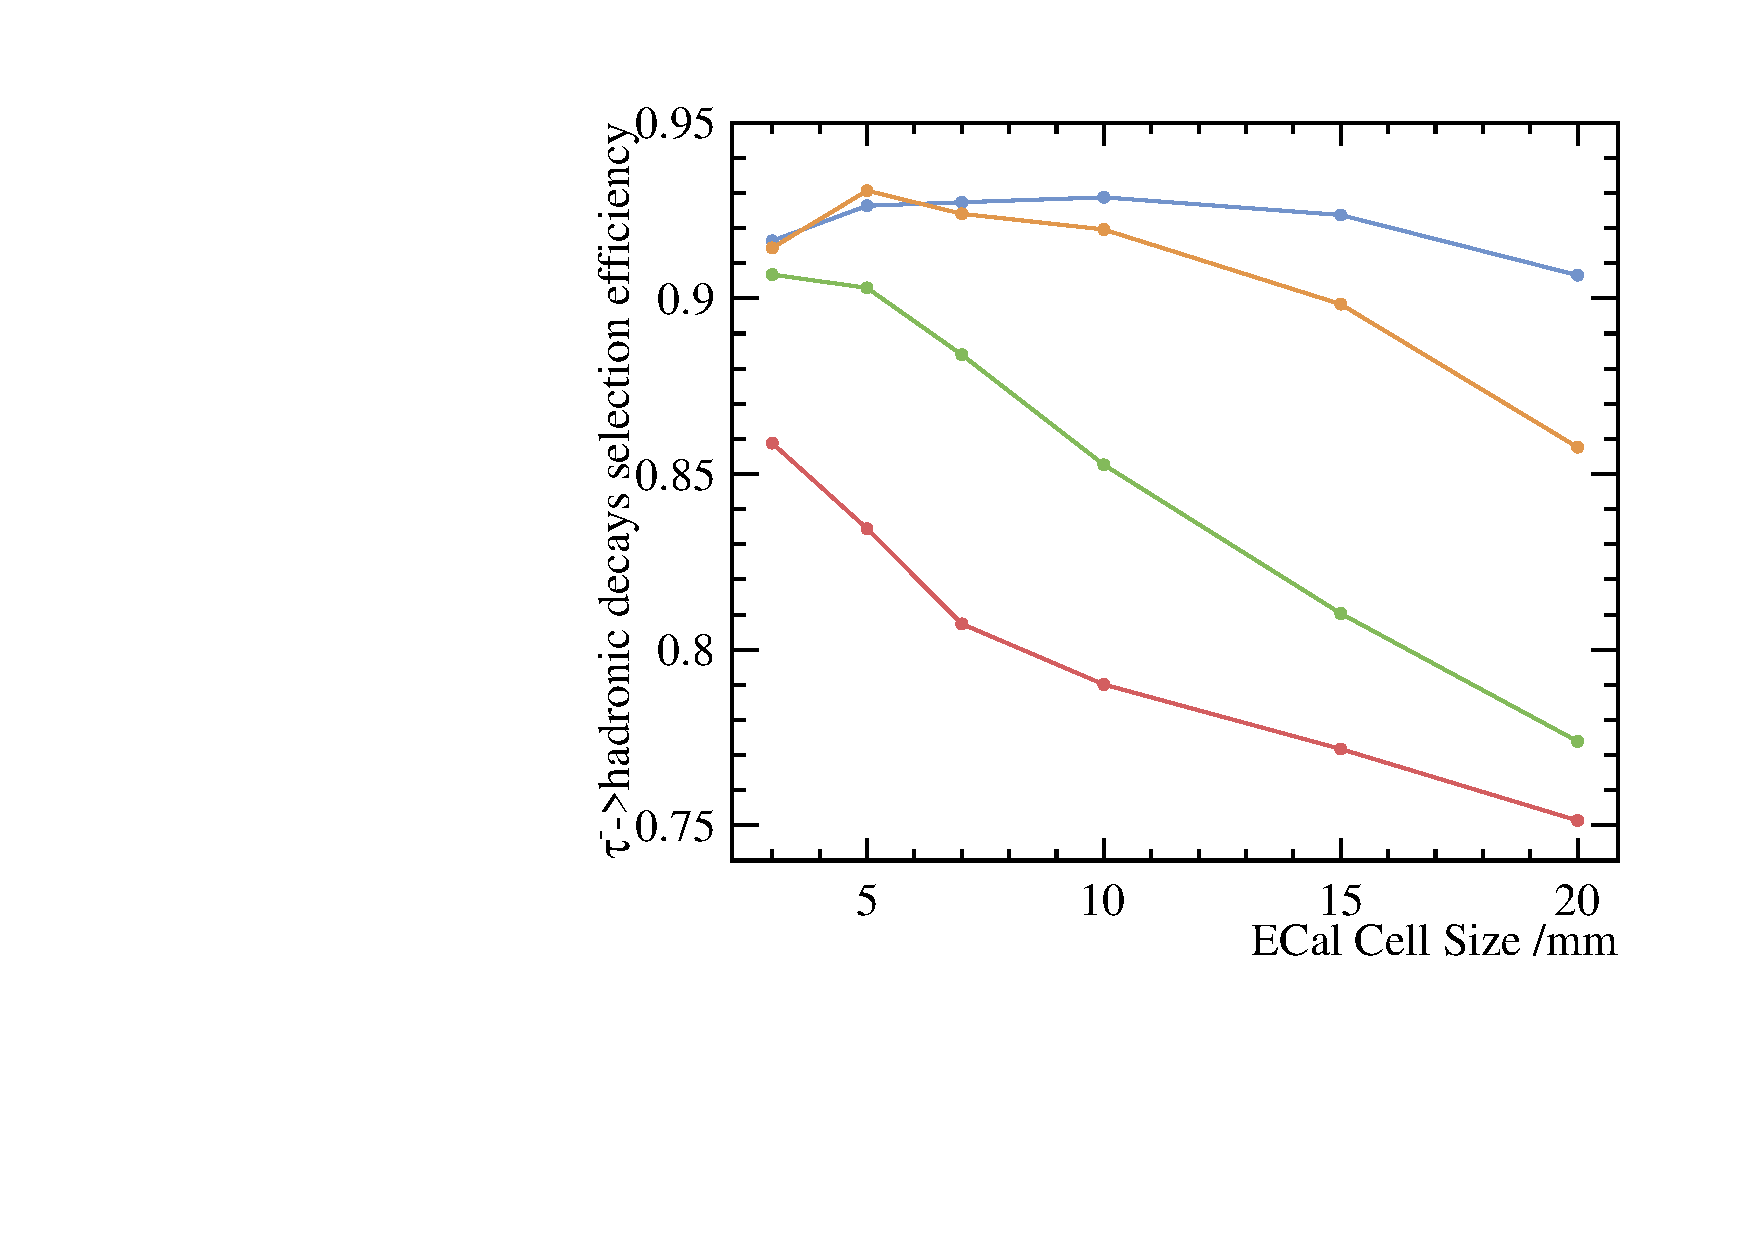
\includegraphics[width=.4\textwidth]{plots/hadEff}
% "\includegraphics" from the "graphicx" permits to crop (trim+clip)
% and rotate (angle) and image (and much more)
\caption[]%
{The selection efficiencies for various final states against the ECal cell size for different c.o.m. energies with the nominal \CLICILD detector model are shown. The top left, top right, middle left, middle right and bottom left plots are for the \decayPion, \decayRho,  \decayAiPhoton, \decayAiPion  and \decayThreePionPhoton  final states respectively. From the top to the bottom, blue, orange, green and red lines are representing the \sqrtS = 100, 200, 500 and 1000\,GeV respectively.}
\label{fig:TauPionEfficiency}
\end{figure}

To access the impact different ECal square size on detector performance, in particular ECal performance, the correct reconstruction efficiency for 1-prong and 3-prong final states is used as metric. The higher \sqrtS of the collision would degrade the performance, as photons are more boosted and more difficult to resolve.

The leptonic decay  correct reconstruction efficiency is not used as a metric as they are similar across different ECal cell sizes. This is because the \Pepm and \Pgmpm identifications mostly rely on the tracking system, which was not varied in this study. The energy deposited in the calorimeter are used for the association to the tracks but it has a small impact on the lepton identification.

\Figure{fig:TauPionEfficiency} shows that as the ECal cell sizes increase, the reconstruction efficiencies generally decrease. Larger cell sizes have lower spatial resolutions, making the separating of nearby photons more difficult.

For the \decayAiPhoton final state, the selection efficiency for 500\,GeV rises from ECal cell sizes 15\,mm to 20\,mm and the one for 1000\,GeV rises from 7\,, to 20\,mm actually goes up as cell size increases. This is because when the algorithm can not reconstruct four photons in the \decayAiPhoton final state, and the event topology would be very similar to the \decayRho final states.

For the \rootS = 100 and 200\,GeV, the selection efficiency of the 5\,mm ECal cell size is better than that of the 3\,mm. One possible explanation is that the  and the PandoraPFA have been optimised for the nominal ILD detector with the 5\,mm ECal cell size, which shares the same ECal structure with the nominal \CLICILD detector.


\begin{figure}[htbp]
\centering % \begin{center}/\end{center} takes some additional vertical space
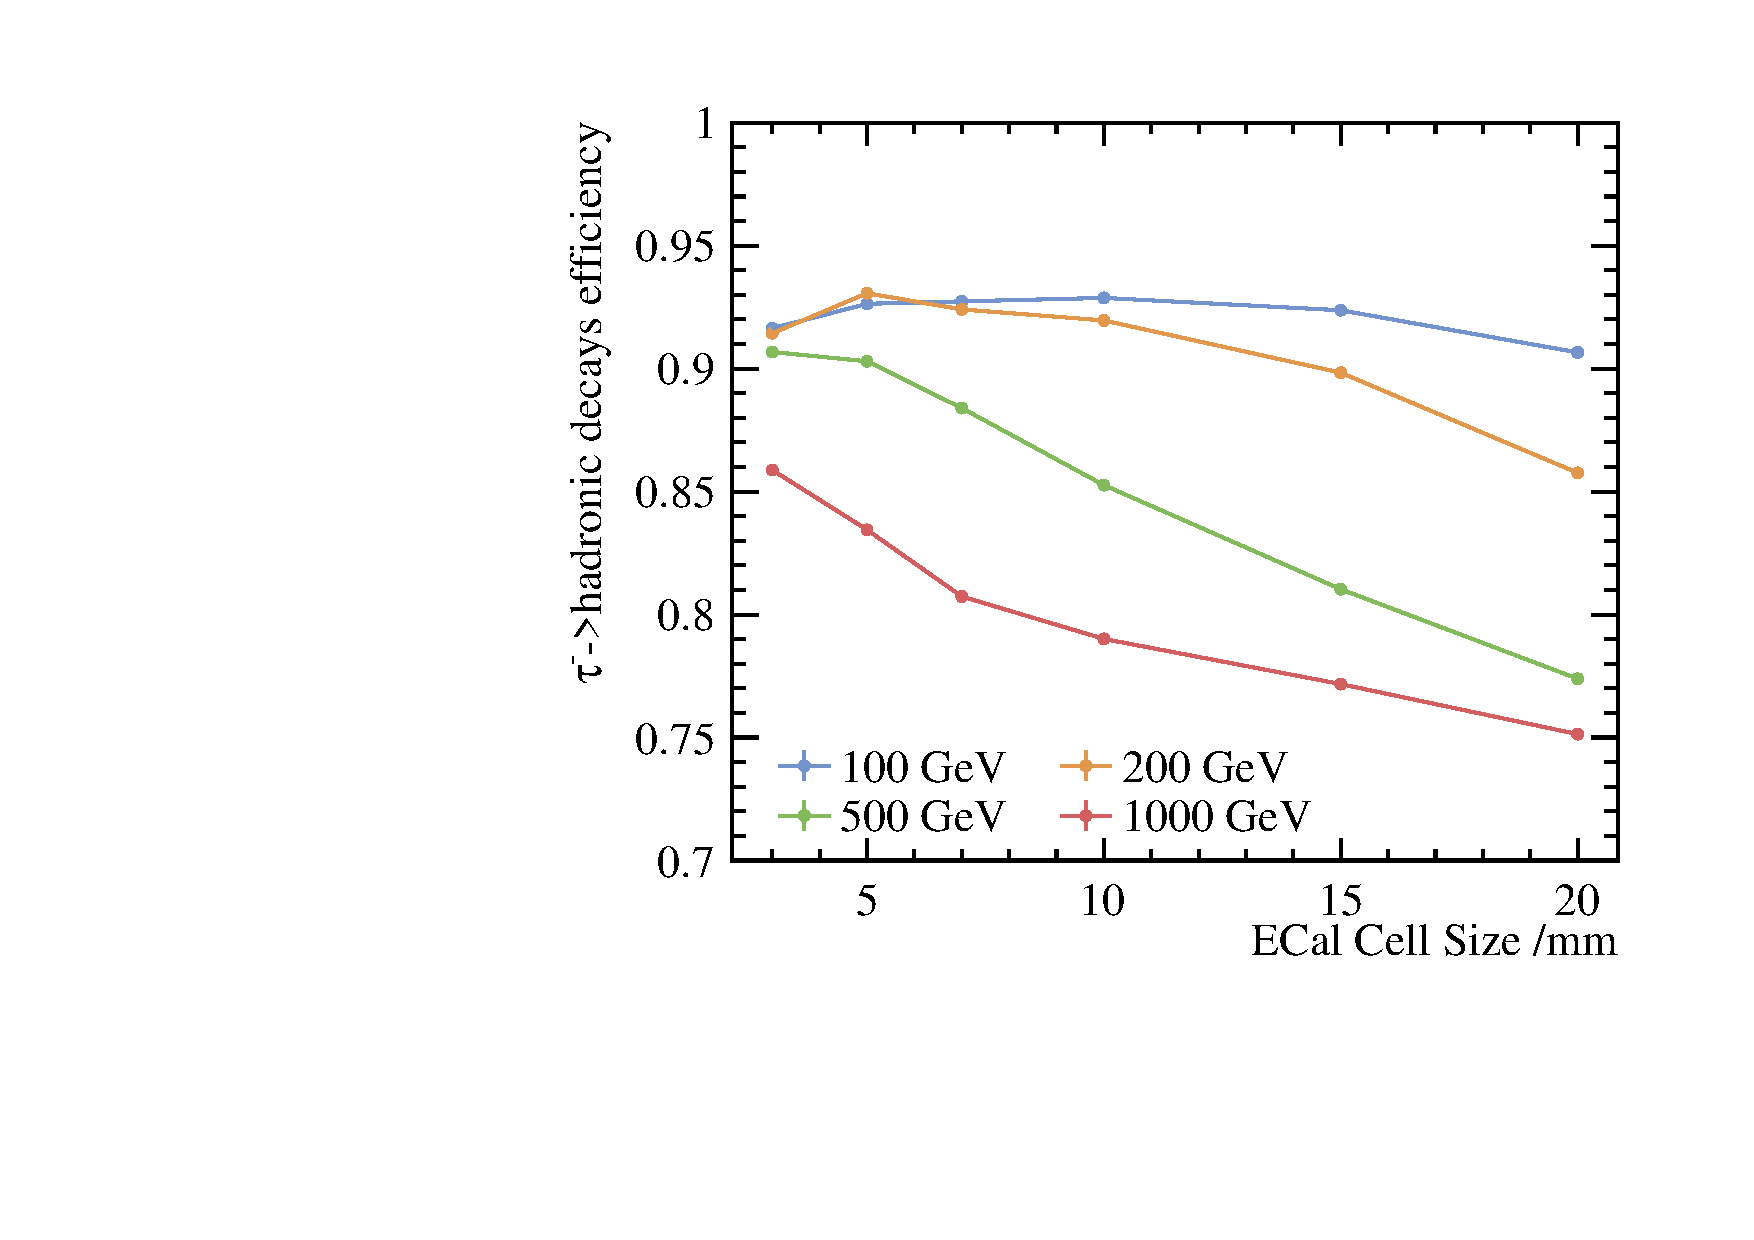
\includegraphics[width=.45\textwidth]{tau/hadronicEff}
% "\includegraphics" from the "graphicx" permits to crop (trim+clip)
% and rotate (angle) and image (and much more)
\caption[]%
{The \Pgt hadronic decay efficiency against the ECal cell size for different \rootS energies with the nominal CLIC\_ILD detector model are shown. The blue, orange, green and red lines are representing the \sqrtS = 100, 200, 500 and 1000\,GeV respectively.}
\label{fig:TauHadronicEfficiency}
\end{figure}


To effectively compare the overall separation power of all hadronic final states across \sqrtS and ECal square cell sizes, we constructed a single parameter function, the  \Pgt hadronic decay final state efficiency function,
\begin{equation}
\label{eq:had}
\tauHad = \frac{\Sigma_{i} {Br}_{i}\varepsilon_{i}}{\Sigma_{i} {Br}_{i}}  \,,
\end{equation}

where $Br_{i}$ is the branching fraction of a hadronic final state after the generator level cut. $\varepsilon_{i}$ is the correct reconstruction efficiency of the final state, and the $i$ is summing over five hadronic decay final state of \Pgt. Leptonic decays, \decayElectron and \decayMuon, were not included, because the variation of the leptonic decay selection efficiency is small.


In the \Figure{fig:TauHadronicEfficiency}, \Pgt hadronic decay final state efficiency, \tauHad, against the ECal cell size with different \sqrtS is shown. \tauHad decreases when cell sizes increases and when \sqrtS increases.  \tauHad of the 5\,mm ECal cell size is better than that of the 3\,mm for \sqrtS = 100 and 200\,GeV lines possibly due the optimisation of the software for the nominal ILD 5\,mm ECal square cell size.

The \tauHad is above 90\% for the ECal cell size from 3 to 20\,mm for the \rootSGeV{100}. For \rootSGeV{200}, the \tauHad decreases from over 90\% to 86\% for the ECal square cell size from 3 to 20\,mm. The degradation of the \tauHad is more significant for the \sqrtS = 500 and 1000\,GeV, where the \tauHad drops from over 90\% to 77\%  and from 86\% to 75\% respectively, over the same range of ECal square cell size.

For \sqrtS = 100 and 200\,GeV, up to 15\,mm cell sizes of ECal will give a good performance for \Pgt hadronic decay modes separation, and the \tauHad is above 90\%. For \sqrtS = 500 and 1000\,GeV, it is preferential to have a small ECal cell size for a good \Pgt hadronic decay modes separation. There is about 15\% degradation of \tauHad for ECal square cell size from 3 to 20\,mm.

\section{}